\chapter{动态规划之最短路径算法}

\begin{introduction}
	\item Dijkstra算法
	\item Bellman-Ford算法
	%\item 提要3
	%\item 提要4
	%\item 提要5
\end{introduction}


\section{最短路径定义}
给的一个带权重的有向图$G=(V,E)$和权重函数$\omega : E\rightarrow R$,该权重函数将每条边映射到实数值的权重上。图中一条路径$p=<v_0,v_1,...,v_k>$的权重$\omega (p)$是构成该路径的所有边的权重之和:$$\omega (p)=\sum\limit_{i=1}^k\omega (v_{i-1},v_i)$$

定义从结点$u$到结点$v$的最短路径权重


\begin{equation}
\delta(u,v) = \begin{cases}
min( \omega (p) : u\stackrel{p}{\longrightarrow} v )  & uv\text{连通} \notag\\
+\infty   &  uv\text{不连通}

\end{cases}
\end{equation}


从结点$u$到结点$v$的最短路径则定义为任何一条权重为$\omega (p)=\delta(u,v)$的从结点$u$到结点$v$的路径$p$

对于每个节点,我们定义两个属性。v.d用来记录源节点s到节点v的最短路径权重上界。v.f用来记录节点v的前驱节点。

定义初始化和松弛两个操作。

\begin{lstlisting}[caption=初始化和松弛伪代码]
INITIALIZE-SINGLE-SOURCE(G,s)
for each vertex v in G.V
         v.d=$\infty$
    v.f=NULL
s.d=0

RELAX(u,v)
if v.d>u.d+(u,v)
       v.d=u.d+(u,v)
	   v.f=u
\end{lstlisting}

\section{Dijkstra算法}
Dijkstra算法解决的是一般情况下的单源最短路径问题,边的权重要求为非负值。

Dijkstra算法在运行过程中关键是维护一个结点的集合$S$。从源节点$s$到该集合中的每个结点之间的最短路径已经找到。该算法重复
从结点集$V-S$中选择离源节点最近的结点$u$加入到集合$S$中。然后重新计算源节点到其余各点的距离。如此以往,直到所有点都加入到集合$S$中。

\begin{lstlisting}[caption=Dijkstra算法伪代码]
DIJKSTRA(G,S)
INITIALIZE-SINGLE-SOURCE(G,s)
S=NULL
Q=G.V
while Q!=NULL
        u=EXTRACT-MIN(Q)
		S=S+u
		for each vertex v in G.Adj[u]
		         RELAX(u,v)

\end{lstlisting}

算法运行过程如下:

\begin{figure}
\centering
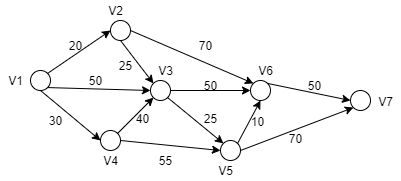
\includegraphics[width=10cm,height=5cm]{image/dijkstra1.png}
\caption{一个带权有向图}
\end{figure}
\begin{figure}
\centering
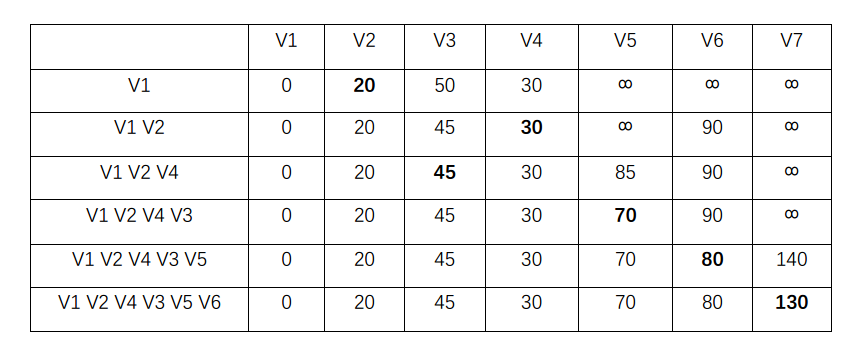
\includegraphics[width=10cm,height=5cm]{image/dijkstra2.png}
\caption{对应Dijkstar算法执行过程表格}
\end{figure}

表的左侧是当前的集合。表中每一行的数字为源点通过集合中的点到各点的当前最短路径距离。在表中加粗的数字对应的节点为该轮中将被加入到集合$S$中节点。

\subsection{时间复杂度}
算法第1行初始化操作所需时间为$\Theta(V)$,第4行循环一共执|V|次,其中第5行操作所需时间为$O(V)$,第7行的for循环在整个算法执行期间一共执行|E|次,故Dijkstra算法的总运行时间为$O(V^2+E)=O(V^2)$

\subsection{正确性证明}
Dijkstra算法使用贪心的策略,每次选择”最近“的节点加入到集合中。下面通过对已经访问的节点数学归纳法证明其正确性。

1. 当只有两个节点的时候,显然成立。

2. 假设n-1个结点时。现在我们选择一条边(v,u),其中节点u是未访问结点中具有最小的u.d的节点,并且$u.d=v.d+\omega(v,u)$。u.d必定是源点到所有未访问中最短路径长度。因为假如有一条更短的路径,假设k是该路径上第一个未访问的节点,这与假设$k.d>u.d$矛盾,所以u.d必定是源点到所有未访问节点中最短路径长度。类似,如果在没有使用未访问节点情况下存在一条到节点u的更短路径,并且如果该路径上最后一个节点是k,则我们有$u.d=k.d+\omega(k,u)$,与前提矛盾。其余未访问节点同理。

综上所述,Dijkstra算法正确。

\section{Bellman-Ford算法}
Bellman-Ford算法解决的是一般情况下的单源最短路径问题,边的权重可以为负值。

由分析可知,s到t的最短路一定是一个简单路径。并且最短路径的边数小于等于n-1(n为节点数)。我们记opt(v,k)为从v到t,边数小于等于k的最短路径。考虑两种情况,一种是最短路径边数小于等于k-1,一种是边数等于k的。
则有
$$opt(v,k)=min(opt(v,k-1),\min \limits_{(v,w)\in E}(opt(w,k-1)+c(v,w)))$$
其中w是与v直接相连的点。

同理还可以记opt(t,k)为从v到t,边数小于等于k的最短路径。则有
$$opt(t,k)=min(opt(t,k-1),\min \limits_{(w,t)\in E}(opt(w,k-1)+c(w,t)))$$

\begin{lstlisting}[caption=Bellman-Ford算法算法伪代码]
BELLMAN-FORD(G,s)

INITIALIZE-SINGLE-SOURCE(G,s)
for i=1 to |G.V|-1
        for each edge(u,v) in G.E
		         RELAX(u,v)
for each edge(u,v) in G.E
         if v.d>u.d+(u,v)
		       return FALSE
return TRUE

\end{lstlisting}

\subsection{时间复杂度}
算法第1行初始化操作所需时间为$\Theta (V)$,第2到4行循环的运行时间为$\Theta (E)$,且一共要进行|V|-1次循环,第5到7行的for循环所需时间为O(E),Bellman-Ford算法的总运行时间为O(VE)。

\subsection{正确性证明}
若某节点和源点不连通,初始化时,除了源点的距离为0外,其他节点的初始化为无穷大。如果不连通,则该节点所在的连通图的任一条边都不会导致更新。

若节点x点与源点连通。每个点都存在自己的最短路,为$(e_0,e_1,e_2,...,e_k)$。显然,源点只要经过|V|-1条边就可到达任一点。

现只需证明,对节点v,每次松弛操作,至少有一条最短边$e_i$的距离被找到,除非已经到达v点。

对于第一次松弛,必定更新和源点s相连的所有出边。由于源点s初始距离是0,和其相连的节点初始距离都是无穷大。而这些相连的出边中,必有一条是节点v的最短路上起始的一条边。则设有节点k,这个节点是节点v最短路上的一共点,由于下一次松弛将更新与k相连的所有点,必能找到下一个点,且也是节点v的最短路径上的一个点。则通过多次松弛可以找出最短路。

综上所述,Bellman-Ford算法正确。
